\begin{figure}[h!]
\centering
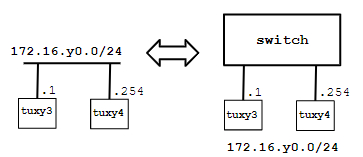
\includegraphics[scale=0.5]{imagens/Exp1.png}
\caption{Arquitetura da Primeira Experiência}
\label{fig:exp1}
\end{figure}

Esta experiência tem como objetivos perceber o que são pacotes ARP e para que servem, que tipo de pacotes é que o comando ping gera e o que são endereços MAC e endereços IP.

Os comandos usados para esta experiência podem ser encontrados no Anexo \ref{exp1_steps}.
\subsubsection{Análise dos Logs}

Pacotes ARP \footnote{Adress Resolution Protocol} são usados para, sabendo o endereço IP \footnote{Internet Protocol} de uma máquina, pedir o endereço MAC \footnote{Medium Access Control}. Os endereços MAC são os identificadores das placas de rede enquanto que os endereços IP servem como identificadores públicos que cada máquina necessita de usar numa rede para poder comunicar com outras máquinas. Uma máquina pode possuir vários endereços IP, mas apenas 1 endereço MAC.

O comando ping gera pacotes ICMP \footnote{Internet Control Message Protocol}. Estes pacotes são normalmente usados por routers ou hosts para mandar erros da camada 3 ou mensagens de controlo para outros routers ou hosts. Nesta experiência o comando ping serve para descobrir se existe conectividade entre computadores.

Ao analisar os logs desta experiência é possível verificar o formato dos pacotes ARP que são enviados quando se faz ping (Figura \ref{fig:arp_packets}), juntamente com os pacotes ICMP de ping (Figura \ref{fig:icmp_packets}). O Wireshark atribui cores diferentes a tipos de pacotes diferentes, mas é possível ver o tipo de pacote nos detalhes dos mesmos (Figuras \ref{fig:arp_wireshark} e \ref{fig:icmp_wireshark}).

Para ver o tamanho de uma trama que é recebida, a partir do wireshark, verifica-se o valor em bytes passados "on wire", ou então, para tramas IPv4, estas possuem um campo "Total Length" com o valor em bytes do tamanho da trama.